%+----------------------------------------------------------+
%| SLIDES: Construction and Reduction of the L-infinity Algebra of Observables
%|         Associated with a BV-Module
%| Contents: - 60 minutes (estimated duration ~2.5 minutes per slide, ~24 slides)
%|
%| Author: Antonio Miti
%| Event: ARTS — Algebra and Representation Theory Seminar
%| Place: Università di Roma  "Tor Vergata "
%| Date: 21/10/2025
%| Link: https://www.mat.uniroma2.it/~ricerca/algebr/page-AREA_files/page-AREA-2_files/talks.html
%+----------------------------------------------------------+



%- HandOut Flag -----------------------------------------------------------------------------------------
	\newif\ifHandout
	\Handouttrue  %uncomment for the printable version
	%Handling of flags it is not preserved when passing to standalone-subfiles!


%- D0cum3nt ----------------------------------------------------------------------------------------------
\ifHandout
	\documentclass[handout,10pt]{beamer}   
	\setbeameroption{show notes} %print notes   
\else
	\documentclass[10pt]{beamer}
\fi


%- Packages ----------------------------------------------------------------------------------------------
\usepackage{custom-style}
\usepackage{math}

%- Bibliography (Biber) ----------------------------------------------------------------------------------
\usepackage[backend=biber,style=alphabetic,maxnames=2]{biblatex}
\bibliography{bibfile.bib}

%- L30's ----------------------------------------------------------------------------------------------
\usepackage{quiver} %https://q.uiver.app/ % Not in Miktex!
\usetikzlibrary{nfold}
\usetikzlibrary{decorations.pathmorphing} 
\renewcommand{\Ham}{\mathrm{Ham}}
\newcommand{\Der}{\mathrm{Der}}
\usepackage{enumitem}
\setlist{topsep=0pt, leftmargin=*,label=$\bullet$}


%--Beamer Style-----------------------------------------------------------------------------------------------
\usetheme{toninus}

\usetikzlibrary{backgrounds}
  \tikzset{
    invisible/.style={opacity=0},
    visible on/.style={alt=#1{}{invisible}},
    alt/.code args={<#1>#2#3}{%
      \alt<#1>{\pgfkeysalso{#2}}{\pgfkeysalso{#3}} % \pgfkeysalso doesn't change the path
    },
  }


%- T1tle P4g3 -------------------------------------------------------------------------------------------
\title{Construction and Reduction of the $L_\infty$ Algebra of Observables Associated with a BV-Module} 
\subtitle{\href{https://www.mat.uniroma2.it/~ricerca/algebr/page-AREA_files/page-AREA-2_files/talks.html}{- ARTS - Algebra and Representation Theory Seminar in Roma "Tor Vergata"}}
\author[AMM]{
	\href{https://www.antoniomiti.it/}{Antonio Michele Miti}
	{\small joint work w/ Leonid Ryvkin}
}
\institute[SUR]{
	Sapienza Università di Roma \\
	Rome, Italy 	\\
	\vspace{.5em}
  \begin{tabular}[h]{ccc}
      \href{https://www.mat.uniroma1.it/en}{
\includegraphics[width=6cm]{./Logos/Sur_logo}} & & 
      \href{https://civis3i.univ-amu.fr/en/civis3i-alliance-programme}{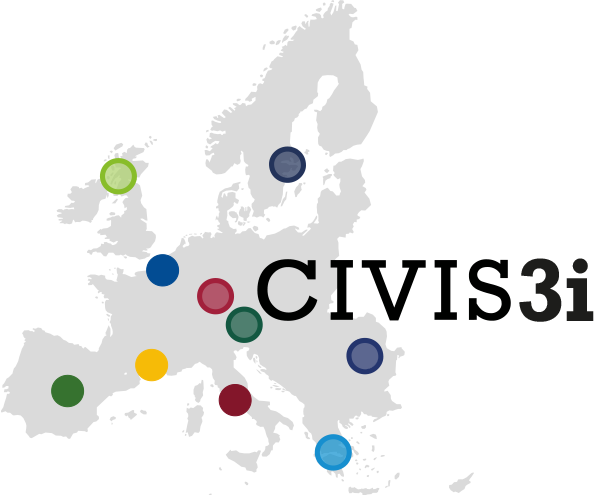
\includegraphics[width=3cm]{Logos/Civis_logo}}
  \end{tabular}    
}
\date[TorV25] % (optional, should be abbreviation of conference name)
{	
	{\vskip 1ex}
	Universit\'a di Roma - Tor Vergata, October 2025
}



%+----------------------------------------------------------+
%- D0cum3nt ------------------------------------------------+
%+----------------------------------------------------------+
\begin{document}
%+----------------------------------------------------------+





\begin{frame}
  \titlepage
\end{frame}

%+----------------------------------------------------------+
% S3cti0n: Intr0ducti0n ------------------------------------+
\section{Introduction}
%+----------------------------------------------------------+
%

\begin{frame}{Symplectic Geometry}
\begin{itemize}
  \item Symplectic manifold: $(M,\omega)$ with $\omega$ closed, nondegenerate 2-form.
  \item Observables: $C^\infty(M)$ with Poisson bracket $\{f,g\} = \omega(X_f, X_g)$.
  \item $X_f$ is the Hamiltonian vector field: $\iota_{X_f} \omega = df$.
\end{itemize}
\end{frame}
\note{Symplectic vs. Multisymplectic Geometry: In symplectic geometry, a closed nondegenerate 2-form $\omega$ on a manifold $M$ gives rise to a Poisson algebra of observables (smooth functions with the Poisson bracket) . In contrast, multisymplectic manifolds carry a closed nondegenerate form of degree $>2$ (often called an $n$-plectic form if its degree is $n+1$). These higher-degree forms naturally lead not to a Poisson Lie algebra, but to a higher (homotopy) Lie algebra structure on observables. In fact, as shown by Rogers, an $n$-plectic manifold yields an $n$-term $L_\infty$-algebra of observables (sometimes called a higher Poisson algebra) .org. This generalizes the Poisson bracket: for example, a 3-plectic form (degree 3) gives a Lie 2-algebra of observables, etc., with higher multi-brackets capturing the failure of the Jacobi identity up to homotopy.

Symplectic Case: If $(M,\omega)$ is a symplectic manifold (closed nondegenerate 2-form), every smooth function $f\in C^\infty(M)$ has an associated Hamiltonian vector field $X_f$ defined by $i_{X_f}\omega = d f$. The space of observables $C^\infty(M)$ forms a Poisson algebra with the Poisson bracket ${f,g} = \omega(X_f, X_g)$. This is just a Lie algebra (indeed a Lie derivation algebra on $C^\infty(M)$) satisfying the Jacobi identity strictly.

}

\begin{frame}{From Symplectic to Multisymplectic}
\begin{itemize}
  \item $k$-plectic manifold: $(M,\omega)$ with closed, nondegenerate $(k+1)$-form.
  \item Hamiltonian $(k-1)$-form $\alpha$: $\iota_X \omega = d\alpha$.
  \item Rogers (2010): observables form an $L_\infty$-algebra.
\end{itemize}
\end{frame}
\note{- **Multisymplectic (Higher-Degree) Forms:** Now let $(M,\omega)$ be a **$k$-plectic manifold**, i.e. $\omega$ is a closed, nondegenerate $(k+1)$-form (for example, a 3-form if $k=2$). The notion of *Hamiltonian observables* generalizes: a **Hamiltonian $(k-1)$-form** $\alpha \in \Omega^{k-1}(M)$ is one that admits a vector field $X$ (a *Hamiltonian field*) satisfying $i_X\omega = d\alpha$. We call the pair $(X,\alpha)$ a *Hamiltonian pair*. Just as in the symplectic case $(k=1)$ where $\alpha$ is a 0-form (function) and $X$ its Hamiltonian vector field, here $\alpha$ plays the role of the observable (often called an $(k-1)$-form observable). The collection of all such Hamiltonian forms (for various degrees) can be organized into a graded object, and Rogers showed that it carries a canonical **$L_\infty$-algebra structure** .
    - **Example:** For a 3-plectic manifold (degree 3 form $\omega$), one has Hamiltonian 1-forms: each 1-form $\alpha$ for which there exists $X$ with $i_X\omega = d\alpha$. These Hamiltonian pairs $(X,\alpha)$ form the degree-0 part of the observables. In addition, ordinary functions (0-forms) can be viewed as Hamiltonian 0-forms (with $X$ such that $i_X\omega = d(0) = 0$), and perhaps higher-degree observables appear up to degree 1 in this case. The resulting $L_\infty$ has non-trivial brackets of arity up to 2 (making it a *Lie 2-algebra* of observables, a kind of higher Poisson algebra). The 2-bracket extends the Poisson bracket, and a 3-bracket arises measuring the failure of the Jacobi identity (something that vanishes in the symplectic case but not in general). For a 4-plectic form, one would get a Lie 3-algebra, etc.}

\begin{frame}{$L_\infty$ Algebra of Observables}
\begin{itemize}
  \item Observables organized as graded vector space: Hamiltonian forms + multi-brackets.
  \item Higher brackets from Cartan calculus: $d$, $\iota_X$, $L_X$.
  \item No manifold needed if we have the algebraic structure.
\end{itemize}
\end{frame}
\note{Rogers’ Construction (2010/2012): The remarkable insight of Rogers  was that the construction of this observables $L_\infty$-algebra is essentially algebraic, relying only on the standard Cartan calculus identities for differential forms and vector fields. In other words, Rogers’ $L_\infty$ brackets can be derived from the algebraic relations between the exterior derivative $d$, the interior product $i_X$, and the Lie derivative $L_X$ on forms . This suggests we can abstract and generalize the construction beyond the category of manifolds. The goal is to build an $L_\infty$-algebra of observables in a purely algebraic setting, provided we have an analog of  "forms " and  "vector fields " satisfying the Cartan relations .}

\begin{frame}{Reminder: What’s an $L_\infty$ Algebra?}
\begin{itemize}
  \item Graded vector space $V = \bigoplus V^i$.
  \item Maps $\ell_k: V^{\otimes k} \to V$ of degree $2 - k$.
  \item Satisfying higher Jacobi identities (homotopy Lie algebra).
\end{itemize}
\end{frame}
\note{- **Higher Brackets via Cartan Calculus:** The construction of the $L_\infty$ brackets can be understood conceptually in terms of the **Cartan calculus identities**. Recall that on a manifold, we have for any vector fields $X,Y$ and differential forms $\alpha$:
    - $L_X = [d, i_X]$ (Cartan’s identity relating Lie derivative and interior contraction), and
    - $[L_X, i_Y] = i_{[X,Y]}$ (compatibility of Lie derivative with contraction),
    - $[L_X,L_Y] = L_{[X,Y]}$, etc. 
        
        These identities ensure that the operations $d, i_X, L_X$ behave in a coordinated way (the essence of *Gerstenhaber algebra and BV-module* structure, as we formalize below). Rogers’ $L_\infty$ brackets are built using these ingredients: e.g., the binary bracket of two Hamiltonian forms $(X,\alpha)$ and $(Y,\beta)$ can be defined as $( [X,Y],; L_X\beta)$ (or plus cyclic terms), and higher brackets involve expressions with $i_{X_i} i_{X_j}\omega$ contracted with another argument, etc., ensuring the homotopy Jacobi identities hold . The key point is that all such formulas **only use the algebraic operations $d,i,L,[\cdot,\cdot]$ and the form $\omega$**. This algebraic nature allows generalization to any context where similar operators exist.
        
- **Limitations of Classical Reduction:** Before moving to the algebraic setup, note that reducing multisymplectic systems geometrically (analogue of Marsden-Weinstein reduction) can be challenging. Classical symplectic reduction requires a Lie group action that is free and proper and a regular value of the moment map; these conditions often fail (especially in field theory or higher form cases). Recent work has approached reduction **algebraically** by focusing on the algebra of observables (functions/forms) with constraints, rather than the quotient of manifolds. This algebraic approach, implemented for multisymplectic manifolds in Blacker-Miti-Ryvkin 2024, allows handling singular cases (non-free actions, etc.) by *encoding constraints and symmetries at the algebraic level.
Our work builds on this idea using *constraint triples*.}

\begin{frame}{Scope/Idea of the Talk}
\begin{itemize}
  \item Generalize Rogers' construction to a purely algebraic setting.
  \item Use Gerstenhaber algebras and BV-modules.
  \item Handle reduction via constraint triples.
  \item Apply to recover and extend results on multisymplectic reduction.
\end{itemize}
\end{frame}
\note{Our Aim: In this talk, we present such a fully algebraic formalism for constructing and reducing $L_\infty$-algebras of observables, inspired by multisymplectic geometryarxiv.org. We work in the framework of Gerstenhaber algebras and Batalin-Vilkovisky modules (BV-modules), which encapsulate the algebraic structure of Cartan calculus (including both commutative and non-commutative cases). Given any Gerstenhaber algebra $G$ together with a BV-module $M$ and a chosen closed element (a  "cocycle ") $c$ in $M$, we will show how to construct an associated $L_\infty$-algebra of observables without reference to any underlying manifold . This is our Theorem A. Moreover, we will address how to perform reduction of these observables $L_\infty$-algebras in the presence of constraints or symmetries. For this, we employ the notion of constraint triples (introduced by Dippel-Esposito-Waldmann 2019marvindippell.de) as an algebraic framework for coisotropic reduction. Adapting this to our BV-module setting, we obtain a general procedure to reduce an $L_\infty$ of observables, even in singular scenarios where classical quotient constructions fail  . This corresponds to Theorem C in our work. In particular, our approach reproduces the multisymplectic reduction results of Blacker-Miti-Ryvkin (SIGMA 2024) in a more conceptual way and clarifies the role of the so-called  "residue defect " that appears in the reduction process .}

%+----------------------------------------------------------+
%Overview: Roughly the first half of the talk will be introductory. We will recall the necessary background on multisymplectic observables and momentum maps, then introduce the algebraic structures (Gerstenhaber algebras and BV-modules) that replicate Cartan calculus. In the second half, we outline the construction of the observables $L_\infty$-algebra in the algebraic setting (Theorem A), and then discuss how to incorporate constraints via constraint triples, leading to a reduced $L_\infty$-algebra of observables (Theorem C). 

%+----------------------------------------------------------+
%Section: BV-Modules ----------------------------------+
\section{BV-Modules: Algebraic Cartan Calculus}
%+----------------------------------------------------------+
%

\begin{frame}{Lie-Rinehart Algebras}
\begin{itemize}
  \item Pair $(A,E)$: $A$ a commutative algebra, $E$ an $A$-module and Lie algebra.
  \item Anchor map: $\rho: E \to \mathrm{Der}(A)$.
  \item Encodes derivations + Lie algebra structure.
\end{itemize}
\end{frame}
\note{To generalize the above geometric structures, we introduce the algebraic counterparts of  "multivector fields " and  "differential forms with Cartan calculus. " All vector spaces are over a field of characteristic 0 (e.g. $\mathbb{R}$). We work in graded settings since forms and multivectors are naturally graded.

- **Lie-Rinehart Algebras:** A *Lie-Rinehart algebra* $(A,E)$ consists of a commutative associative algebra $A$ (think of $A=C^\infty(M)$) and an $A$-module $E$ (think of $E=\mathfrak X(M)$, the vector fields) which is also a Lie algebra, together with an *anchor* map $\rho: E \to \mathop{\mathrm{Der}}(A)$ (derivations of $A$) satisfying a Leibniz rule: $[X, aY] = a[X,Y] + (\rho(X)a),Y$. This abstractly encodes the notion of derivations of $A$ with an $A$-linear Lie bracket. **Example:** If $A=C^\infty(M)$, then $E=\Gamma(TM)$ (the module of vector fields) with the identity anchor $\rho(X)=X$ is a Lie-Rinehart algebra. In fact, Lie-Rinehart algebras are algebraic analogues of Lie algebroids (and every Lie algebroid gives a Lie-Rinehart algebra).}

\begin{frame}{Gerstenhaber Algebras}
\begin{itemize}
  \item Graded commutative algebra $(\mathcal{G}, \wedge)$.
  \item Lie bracket $[\cdot,\cdot]$ of degree $-1$.
  \item Compatibility (Leibniz rule): $[x, y\wedge z] = [x,y]\wedge z + (-1)^{(\deg x -1)\deg y} y\wedge [x,z]$.
\end{itemize}
\end{frame}
\note{- **Gerstenhaber Algebras:** A *Gerstenhaber algebra* is a graded algebra that captures the structure of *exterior algebra of multivector fields*. Formally, it is a triple $(\mathcal{G}, \wedge, [\cdot,\cdot])$ where:
    - $\mathcal{G} = \bigoplus_{i\in\mathbb{Z}} \mathcal{G}^i$ is a $\mathbb{Z}$-graded vector space.
    - $\wedge: \mathcal{G}^p \times \mathcal{G}^q \to \mathcal{G}^{p+q}$ is a graded-commutative, associative product (degree $0$ operation).
    - $[\cdot,\cdot]: \mathcal{G}^p \times \mathcal{G}^q \to \mathcal{G}^{p+q-1}$ is a bracket of degree $-1$, making $\mathcal{G}$ into a graded Lie algebra.
    - **Compatibility (Leibniz rule):** The bracket is a derivation of the product: $[x, y\wedge z] = [x,y]\wedge z + (-1)^{(deg,x -1),deg,y} ,y\wedge [x,z]$ for homogeneous $x,y,z$. This is the defining Gerstenhaber identity, generalizing the fact that the Lie bracket of vector fields satisfies a Leibniz rule with respect to wedge of forms or functions.
    
    **Example:** If $(A,E)$ is a Lie-Rinehart algebra, the **exterior algebra** of $E$ (with a degree shift) carries a natural Gerstenhaber structure. In particular, take $\mathcal{G} = \Lambda^\bullet E$ (the exterior *wedge* algebra of $E$ treated as a graded space of multivectors). The wedge product is the usual wedge of multivectors, and the bracket is the **Schouten-Nijenhuis bracket** extending the Lie bracket on $E$ to all multivectors. This $(\Lambda E,\wedge,[\cdot,\cdot]_{SN})$ is a Gerstenhaber algebra, prototypical in geometry (for $E=\mathfrak X(M)$ one recovers the standard Gerstenhaber algebra of multivector fields on $M$).}

\begin{frame}{Gerstenhaber Modules}
\begin{itemize}
  \item $G$-module $M$ with contraction $\iota_X$ of degree $-\deg X$.
  \item Induced Lie derivative $L_X = [d,\iota_X]$ when $d$ is defined.
\end{itemize}
\end{frame}
\note{Gerstenhaber Module: Given a Gerstenhaber algebra $G$, a Gerstenhaber $G$-module is a graded module $M = \bigoplus M^i$ equipped with an action of $G$ that extends the idea of a multivector acting on forms by contraction. Concretely, for each element $X\in G^p$, we have a degree $-p$ operator $i_X: M^\ast \to M^{\ast-p}$ (interpreted as interior product by $X$) satisfying a compatible set of identities (graded derivations, etc.)ar5iv.labs.arxiv.org. We also typically get an induced Lie derivative action $L_X$ of degree 0 defined by $L_X := [D,;i_X]$ once a differential $D$ is present (see below). We won’t detail the full set of axioms here, but essentially a Gerstenhaber module gives an algebraic version of the pair of operations $(i_X, L_X)$ acting on a  "forms " module, with $i$ being antiderivations and $L$ Lie derivations. (The literature sometimes refers to this structure as a  "TTN (Tsygan-Tamarkin-Nest) calculus " .)}

\begin{frame}{BV-Modules}
\begin{itemize}
  \item A Gerstenhaber module $M$ with differential $d$.
  \item Cartan identity: $L_X = [d,\iota_X]$.
  \item Encodes full algebraic Cartan calculus.
\end{itemize}
\end{frame}
\note{Batalin-Vilkovisky Modules (BV-Modules): A BV-module is a Gerstenhaber module that is also equipped with a differential of degree $+1$ (like an exterior derivative) satisfying Cartan’s formula. Formally, let $G$ be a Gerstenhaber algebra and $(M,d)$ a cochain complex (so $d: M^i \to M^{i+1}$ with $d^2=0$). We say $M$ is a BV-module over $G$ if $M$ is a Gerstenhaber $G$-module and, for all $X\in G$, we have the Cartan identity $L_X = [d,; i_X]$ (and automatically $[L_X, i_Y] = i_{[X,Y]}$, etc.)  . In other words, $M$ carries an action of $G$ by contraction $i_X$ and Lie derivative $L_X$ such that together with the differential $d$ they satisfy the standard graded commutation relations of Cartan calculus. We often call $d$ the BV differential.}

\begin{frame}{Abstract Cartan Calculus}
\begin{itemize}
  \item $(G,M,d)$ with $G$ Gerstenhaber, $M$ BV-module, $d^2=0$.
  \item Examples: $(\mathfrak{X}^\bullet(M),\Omega^\bullet(M), d)$.
  \item Extends to noncommutative and algebraic settings.
\end{itemize}
\end{frame}
\note{Example (Classical Cartan Calculus): Take $G = \Lambda^\bullet \mathfrak X(M)$ (Gerstenhaber algebra of multivector fields on a manifold) and $M=\Omega^\bullet(M)$ (the de Rham complex of differential forms). This is a canonical example of a BV-module  : the differential $d$ is the exterior derivative, the contraction $i_X$ is the usual insertion of a multivector $X$ into a form, and the Lie derivative $L_X$ is the usual one acting on forms. These satisfy $L_X = d \circ i_X + i_X \circ d$ (Cartan formula) and all other Cartan identities. In fact, this example exactly recovers the classical Cartan calculus on $M$ as a BV-module structure on $\Omega^\bullet(M)$, with $G$ playing the role of  "polyvector fields " . This justifies the abstractions: any Gerstenhaber algebra + BV-module pair can be seen as a generalized  "space of multivectors and forms " with a full Cartan calculus available . We emphasize that such structures exist in much more general settings, including noncommutative geometry (where $A$ is a noncommutative algebra and one considers analogues of forms and multivectors  ), but for our purposes we stick to the algebraic axioms.}


%+----------------------------------------------------------+
%Section: L-infinity Algebra Associated with a BV-Module ---+
%
\section{$L_\infty$ Algebra Associated with a BV-Module}
%+----------------------------------------------------------+
%

\begin{frame}{Hamiltonian Pairs}
\begin{itemize}
  \item Data: $G$, $M$ BV-module, $c \in M$ closed.
  \item Pair $(X,m)$ with $\iota_X c = d m$.
  \item Generalizes $(X_f, f)$ in symplectic geometry.
\end{itemize}
\end{frame}
\note{Given an algebraic Cartan calculus as above, we can now construct the $L_\infty$-algebra of observables in complete generality. The construction mirrors the one Rogers gave on manifolds, but now in purely algebraic terms.

- **Data:** Let $G$ be a Gerstenhaber algebra, $M$ a BV-module over $G$ with differential $d$, and let $c \in M^k$ be a fixed *cocycle*, meaning $d c = 0$. 
Think of $c$ as the algebraic analog of a closed multisymplectic form (indeed in geometry $c$ could be $\omega$, which is closed by assumption). We also assume $c$ is *nondegenerate* in the sense that it induces the relevant pairings (this is automatic in the geometric case and can be treated as a cocycle condition in the algebraic case; for simplicity, we proceed assuming $c$ behaves like a  "volume form " or  "top form " to contract with).
- **Hamiltonian Pairs:** We define a **Hamiltonian pair** as a pair $(X, m)$ with $X \in G$ (a multivector) and $m \in M$ (an element of the module) such that $X$ and $m$ are related by the cocycle $c$ via:

    $i_X(c) = d m$.

    In other words, $m$ is an element whose BV-differential equals the contraction of $c$ with $X$. This is directly analogous to the condition $i_{X_f}\omega = d f$ in the geometric case (here $X$ plays the role of $X_f$ and $m$ plays the role of the observable like $f$ or $\alpha$). We denote by $\mathsf{Ham}(G,M;c)$ the set of all Hamiltonian pairs. In graded terms, one typically considers homogeneous $X$ and $m$ of complementary degrees summing to $k-1$ (so that $i_X c$ has the same degree as $d m$).
    
    **Intuition:** A Hamiltonian pair $(X,m)$ means that $m$ is an *observable* whose  "derived bracket " with the cocycle $c$ yields $X$. If $c$ is nondegenerate, $X$ is uniquely determined by $m$ (just as a symplectic form gives a unique $X_f$ for each $f$), so we can think of $m$ as the *observable element* and $X$ as its *Hamiltonian generator*. However, in singular or degenerate cases, there could be multiple $X$ for a given $m$ or vice versa, hence it is safer to keep the pair. (In the construction we actually consider an appropriate quotient to identify pairs that give the same physical observable; more formally $\mathsf{Ham}(G,M;c)$ can be constructed as a fiber product $G \times_{M} M$ via the maps $X \mapsto i_X c$ and $m \mapsto d m$ .)}

\begin{frame}{The Space and the Multibrackets}
\begin{itemize}
  \item Graded space $\mathcal{O}(G,M;c)$.
  \item Brackets $\ell_k$ built from $d$, $\iota_X$, $L_X$, $[\cdot,\cdot]$.
  \item $\ell_1 = d$, $\ell_2 = $ Lie + derived terms, $\ell_3 = i_{X_1}i_{X_2}i_{X_3}(c)$.
\end{itemize}
\end{frame}
\note{- \textbf{Graded observables space:} We assemble the observables into a graded vector space as follows.

\[
\mathcal{O}(G,M;c)\;=\;\bigoplus_{j\ge 0}\mathcal{O}^j,
\]

where:

- $\mathcal{O}^0$ (degree~0 part) is the space of Hamiltonian pairs $(X,m)$ as above (with $i_X c = d m$).
- For higher degrees $j>0$, roughly speaking $\mathcal{O}^j$ consists of elements of $M$ of degree $(k-1+j)$ (or related shifts) corresponding to forms of lower degree than $c$. In fact, in Rogers' original construction for an $n$-plectic manifold, the $L_\infty$-algebra of observables was an $n$-term complex concentrated in degrees $0,1,\dots,n-1$. Here $k=n+1$ (degree of $c$), so one can show $\mathcal{O}(G,M;c)$ is concentrated in degrees $0$ up to $n-1$ (i.e. $0$ up to $k-2$). Degree~0 are Hamiltonian $(n-1)$-forms (with vector fields), degree~1 would be Hamiltonian $(n-2)$-forms, ..., up to degree $n-1$ corresponding to Hamiltonian $0$-forms (basic observables). We will not need the explicit formula for each degree in this talk; the key is that this graded space includes all would-be observables and their "Hamiltonian partners."}

\begin{frame}{Examples}
\begin{itemize}
  \item Classical: $G=\mathfrak{X}^\bullet(M)$, $M=\Omega^\bullet(M)$, $c=\omega$.
  \item Recovers Rogers’ multisymplectic $L_\infty$.
  \item Other contexts: algebraic, noncommutative, etc.
\end{itemize}
\end{frame}
\note{- **$L_{\infty}$-Algebra Structure:** **Theorem A** (Miti-Ryvkin 2025) states that under the above setup, $\mathcal{O}(G,M;c)$ carries a natural structure of an $L_\infty$-algebra (homotopy Lie algebra) whose brackets are defined using the data of the Gerstenhaber algebra $G$, the BV-module operations, and the cocycle $c$ . Concretely, the multilinear $L_\infty$ operations $\ell_r: \mathcal{O}^{\otimes r} \to \mathcal{O}$ (of degree $2-r$) are given by formulas analogous to those in the multisymplectic manifold case :
    - The unary bracket $\ell_1$ (degree $+1$ map) is essentially induced by the BV differential $d$ on the observable part (it maps a degree~1 element to degree~0 by $\ell_1(m) = (X,d m)$ or something similar, and is zero on degree~0 pairs in the fully nondegenerate case).
    - The binary bracket $\ell_2((X_1,m_1), (X_2,m_2))$ has a result in degree~0 and is given by

        \[
        \ell_2((X_1,m_1),(X_2,m_2)) \;=\; \big([X_1,X_2],\; L_{X_1}m_2 * (-1)^{|X_1|\cdot|X_2|}L_{X_2}m_1\big),
        \]

        which in the simplest case recovers the Poisson bracket structure (when $m$’s are functions, $L_{X_1}m_2 = X_1(m_2)$). The precise formula involves appropriate Koszul signs for graded elements .
        
    - A tertiary bracket $\ell_3((X_1,m_1),(X_2,m_2),(X_3,m_3))$ can be defined using the cocycle $c$: essentially one can take $i_{X_1}i_{X_2}i_{X_3}(c)$ (which is an element of $M$) as part of the output (this corresponds to evaluating the 3-form on three vector fields to get a number or top-form), ensuring that the Jacobi identity holds up to homotopy.
    - Higher brackets $\ell_r$ for $r>3$ may be zero or determined similarly by $c$ if its degree is larger. In fact, for an $(n+1)$-form $c$, all brackets $\ell_r$ with $r> n$ will vanish (so the $L_\infty$ is  "finite " or $n$-term) .
    
    The upshot is that **all these brackets are built out of the operations $[\cdot,\cdot]$ in $G$, $i_X$, $L_X$, $d$, and contraction with $c$**, mimicking the standard formulas in coordinates. It is nontrivial but true that these operations satisfy the required homotopy Jacobi identities. The verification is essentially a translation of Rogers’ original proof to this abstract setting - since Rogers’ proof was  "purely algebraic in nature, " it adapts directly here . We have thus constructed an **$L_\infty$-algebra of observables** $\mathcal{O}(G,M;c)$ associated to any BV-module with a cocycle. This is the main result of the first part of the talk.

    Example (Geometric Case): If we take $G = \Lambda^\bullet \mathfrak X(M)$, $M = \Omega^\bullet(M)$ (so classical Cartan calculus on a manifold), and $c = \omega$ an $n$-plectic form, then $\mathcal{O}(G,M;c)$ precisely recovers Rogers’ $L_\infty$-algebra of observables on $(M,\omega)$  . In degree 0, $\mathcal{O}^0$ consists of Hamiltonian $(n!-!1)$-forms (with their Hamiltonian vector fields), which are exactly Rogers’ observables. The brackets $\ell_r$ coincide with those defined by Rogers (up to sign conventions), and one can check the $L_\infty$ identities by the same calculations in Cartan calculus . This generality shows the power of the BV-module approach: any example of a Gerstenhaber algebra + cocycle yields such an $L_\infty$. For instance, one could even take noncommutative analogues (with a suitable cyclic cocycle playing the role of $c$) to get  "$L_\infty$-observables " in noncommutative geometry  , although we won’t explore that in this talk.}


%+----------------------------------------------------------+
%S3cti0n: An Applicati0n: Multisymplectic Reducti0n -------+
%
\section{An Application: Multisymplectic Reduction}
%+----------------------------------------------------------+
%

\begin{frame}{Constraint Triples}
\begin{itemize}
  \item Triple $(A, A_C, \overline{A})$ with inclusion/projection.
  \item $A_C$ encodes constraints, $\overline{A} = A/I$ reduced algebra.
  \item Adapted to Gerstenhaber and BV-module settings.
\end{itemize}
\end{frame}

\begin{frame}{Constraint BV-Modules}
\begin{itemize}
  \item Triples $(G, G_C, \overline{G})$, $(M, M_C, \overline{M})$.
  \item Structures compatible with Cartan calculus.
  \item Closed cocycle triple $c = (c, c_C, \overline{c})$.
\end{itemize}
\end{frame}

\begin{frame}{Constraint $L_\infty$ Algebra Associated with…}
\begin{itemize}
  \item Construct observables $\mathcal{O} = (\mathcal{O}, \mathcal{O}_C, \overline{\mathcal{O}})$.
  \item Each component carries an $L_\infty$ structure.
  \item Brackets compatible with inclusions/projections.
\end{itemize}
\end{frame}

\begin{frame}{Reduction Functor}
\begin{itemize}
  \item Quotient part $\overline{\mathcal{O}}$ inherits $L_\infty$ structure.
  \item Encodes reduced observables algebra.
  \item No need for regular quotient at geometric level.
\end{itemize}
\end{frame}

\begin{frame}{Recovering Old Results}
\begin{itemize}
  \item Applies to multisymplectic reduction (Blacker-Miti-Ryvkin 2024).
  \item Explains residue defect in homotopy Jacobi identity.
  \item Matches geometric reduction under regularity.
\end{itemize}
\end{frame}

\begin{frame}{Conclusion / Summary}
\begin{itemize}
  \item Algebraic formalism for $L_\infty$ observables via BV-modules.
  \item Generalizes Rogers' result.
  \item Enables reduction via constraint triples.
\end{itemize}
\end{frame}

\begin{frame}{Outlook}
\begin{itemize}
  \item Homotopy momentum maps.
  \item Operadic reformulation.
  \item Applications to field theory.
\end{itemize}
\end{frame}


%+----------------------------------------------------------+
\end{document}
%+----------------------------------------------------------+



We now turn to the second main part: **reduction** of the $L_\infty$-algebra of observables in the presence of constraints or symmetries. In symplectic geometry, reduction is accomplished by the Marsden-Weinstein quotient: one restricts to the zero level set of a momentum map and then quotients by the symmetry group. Algebraically, this corresponds to first imposing ideal relations (for the constraints) and then modding out by gauge symmetries. The **constraint triple** formalism packages these two steps (subobject and quotient) in a single algebraic structure .

- **Constraint Triples:** A **constraint triple** (or **coisotropic triple**) in general consists of:
    1. An algebra (or other structure) $A$ representing the full system’s observables.
    2. A subalgebra $C \subset A$ representing the *constraints* (for example, functions vanishing on a certain submanifold, or first-class constraint algebra in Dirac’s theory).
    3. A quotient (factor) algebra $\overline{A} = A/ I$ for some ideal $I$ related to $C$, representing the *reduced* algebra of observables after constraints are imposed and quotiented.
    
    These are equipped with structure maps (inclusions and projections) satisfying compatibility conditions (e.g. $I$ is the ideal of relations defining $C$) . Intuitively, one has $C$ as the "constraint algebra" (functions that vanish on the constraint surface) and $\overline{A}$ as the algebra of functions on the quotient of that constraint surface by symmetries. Dippel, Esposito & Waldmann formalized this in the context of Poisson algebras and deformation quantization , showing that many reduction procedures can be understood as functors on such triples.
    
    We adopt this idea in our setting: we will consider **constraint Gerstenhaber algebras** and **constraint BV-modules**, which are triples $(G, G_C, \overline{G})$ and $(M, M_C, \overline{M})$ capturing the full, constraint, and reduced parts of our algebraic Cartan calculus . All the structure (brackets, differentials, etc.) is assumed to exist on each part and to be compatible. For instance, a *constraint Gerstenhaber algebra* means $G$ is a Gerstenhaber algebra, $G_C \subset G$ a subalgebra (constraints), and $\overline{G} = G/G_C$ (some quotient) such that the wedge and bracket operations map triples to triples (roughly $[![G, G]!]$ sends $G_C$ to $G_C$ and induces well-defined operations on the quotient) . Similarly, a *constraint BV-module* $(M, M_C, \overline{M})$ has $M_C$ a submodule (the  "constraints on forms ") and $\overline{M}=M/M_C$ the quotient module, with differential $d$ and contractions $i_X$ etc. respecting the triples (so that, e.g., $d(M_C)\subseteq M_C$ and induces a differential on $\overline{M}$) . This is a bit of structure to keep track of, but conceptually it means we have *Cartan calculus not just on one algebra, but simultaneously on a sub- and a quotient algebra*.
    
    - **Origin in Geometry:** If one has a manifold $M$ with a coisotropic submanifold $C\subset M$ (the constraint surface) and a group $G$ acting with gauge orbits, one can form a *constraint manifold* in the sense of Dippel-Kern 2025 . The algebra of smooth functions on a constraint manifold is exactly a constraint triple $(A, C, \overline{A})$ in which $C$ are the functions vanishing on the constraint surface and $\overline{A}$ functions on the quotient (when nice). Likewise, vector fields tangent to $C$ etc. form a constraint Lie-Rinehart algebra, and so on. Indeed, it has been shown that a **constraint Lie-Rinehart algebra** naturally induces a constraint Gerstenhaber algebra and constraint BV-module structures . So this framework is not lacking examples - it generalizes classical constrained Hamiltonian systems.
- **Constraint $L_\infty$ of Observables:** Once we have constraint versions of $G$ and $M$ **and** a *constraint cocycle* $c = (c, c_C, \overline{c})$ (meaning $c$ lies in $M$, $c_C$ in $M_C$ and $\overline{c}$ is its class in $\overline{M}$, with each closed under their respective differentials), we can perform the same construction as before *in the category of constraint complexes*. That is, we define the **constraint Hamiltonian pairs** as triples $((X, X_C, \overline{X}), (m, m_C, \overline{m}))$ such that $i_X(c) = d m$, $i_{X_C}(c_C) = d m_C$ and these are compatible/projection of the first (so $\overline{X}$ and $\overline{m}$ are the images of $X,m$, etc.) . All such triples form a constraint graded space of observables. **Theorem C** asserts that this constraint observables space carries a **constraint $L_\infty$-algebra** structure . By  "constraint $L_\infty$-algebra, " we mean an $L_\infty$ whose underlying structure is also a triple $(L, L_C, \overline{L})$: there are brackets $\ell_r$ on each of $L, L_C, \overline{L}$, and the inclusion/projection maps intertwine these (so that $L_C$ is an $L_\infty$-subalgebra and $\overline{L}$ the quotient $L_\infty$) . The brackets are defined using the same formulas as in the unconstrained case, applied levelwise to $(G, M, c)$, $(G_C, M_C, c_C)$ and inducing $(\overline{G}, \overline{M}, \overline{c})$ . The $L_\infty$ identities hold simultaneously on each level by the same reasoning as before, thanks to the compatibility of the constraint data.
- **Reduction Functor:** Once we have a constraint $L_\infty$-algebra of observables, *reducing it* means passing to the **quotient part** of the constraint triple. In categorical terms, there is a forgetful functor sending a constraint object $(X, X_C, \overline{X})$ to the quotient $\overline{X}$. When we apply this to the constraint $L_\infty$ of observables, we obtain an $L_\infty$-algebra on $\overline{L}$, which we interpret as the **reduced $L_\infty$-algebra of observables** of the constrained system. Intuitively, this $\overline{L}$ encodes observables that are invariant under the symmetry and defined on the constraint surface (since we mod out those that vanish or differ by constraint terms) . By construction, all the $L_\infty$ brackets descend to $\overline{L}$, so the homotopy Lie structure is well-defined on the quotient. This algebra $\overline{L}$ is the algebraic analog of the Poisson algebra of the reduced phase space in classical reduction, but here it can handle the homotopy brackets arising from a multisymplectic form and even if no nice manifold quotient exists (e.g. in singular cases).
- **Recovery of Known Results:** Our general reduction scheme, when applied to the **geometric case** of a multisymplectic manifold with a group action, reproduces the results of our earlier work (Blacker-Miti-Ryvkin, SIGMA 2024) . In that work, we constructed a reduced $L_\infty$ of observables by more ad-hoc means; now we see it fits into the constraint triple framework. Specifically, given a Lie group $G$ acting on an $n$-plectic manifold $(M,\omega)$ with a covariant momentum map $\mu$ , one can form the constraint triple:
    - $A = $ observables $L_\infty$ on $(M,\omega)$,
    - $A_C = $ those observables that vanish on the constraint (e.g. forms pulled back by $\mu$ setting to zero, etc.),
    - $\overline{A} = $ observables on the reduced space (when $0$ level set mod $G$ is nice, these correspond to forms on the quotient).
    
    Our formalism shows that $\overline{A}$ inherits an $L_\infty$-algebra structure automatically . No assumptions of regularity or freeness are needed in the algebraic approach - even if the quotient is singular, $\overline{A}$ is well-defined as a homotopy algebra. This extends the multisymplectic reduction of Blacker 2021 (which assumed regularity) to a far more general context . Moreover, within our algebraic setting we identify an object called the **residue defect**, which measures the slight difference between naive and actual reduction in the homotopy context. In the earlier work, this residue term appeared somewhat mysteriously to satisfy the homotopy Jacobi identities; here we can interpret it cleanly as arising from the constraint differential and the failure of a certain exactness on the constraint submodule. Our framework **clarifies the role of the  "residue defect "**: it is an intrinsic part of the constraint $L_\infty$ structure that vanishes under appropriate conditions (like when the momentum map level is regular) .
    
- **Summary of Main Results:** We can summarize the main technical results (theorems) as follows:
    - **Theorem A:** *Given any Gerstenhaber algebra $G$ with a BV-module $M$ and a closed element $c\in M$, the graded space of Hamiltonian pairs $\mathcal{O}(G,M;c)$ admits an $L_\infty$-algebra structure (observables algebra), defined by the multilinear maps derived from Cartan calculus.* 
    - **Theorem B:** *If $(A,E)$ is a **constraint** Lie-Rinehart algebra (constraint version of derivations over a constraint algebra $A$), then one naturally obtains a constraint Gerstenhaber algebra and a constraint BV-module $(G, M)$ out of it. (In short, classical constraint manifolds yield constraint Cartan calculus algebraically.)
    - **Theorem C:** *Given a constraint Gerstenhaber algebra and BV-module with a constraint cocycle $c$, one can construct a **constraint** $L_\infty$-algebra of observables. Moreover, its **reduced part** $\overline{\mathcal{O}}$ (the quotient level) is an $L_\infty$-algebra that describes the observables of the reduced system.* 
    
    As an application, Theorem C applied to multisymplectic manifolds with symmetries recovers the reduced $L_\infty$ in  and explains the extra terms (residue defect) in a categorical way .
    

## **Conclusion and Outlook**

We have developed a **purely algebraic toolkit** for constructing and reducing $L_\infty$-algebras of observables, extending concepts from symplectic geometry to multisymplectic and even noncommutative settings . This framework shows the power of combining homotopy algebra (for observables) with constraint category theory (for reduction). It provides a unified perspective where classical geometric reduction is just one instance of an algebraic functor acting on $L_\infty$-algebras .

Some directions for further research include:

- **Homotopy Momentum Maps:** Relating our constraint $L_\infty$-reduction to the notion of *homotopy momentum maps* (which appear in alternative higher reduction approaches, e.g. the work of Callies-Frégier-Rogers-Zambon on $L_\infty$-moment maps . It would be interesting to connect the **Leibniz-algebra-valued momentum maps** used here  with homotopy moment maps in an $L_\infty$-context.
- **Operadic Formulation:** The constraint triple constructions hint at an operadic or higher-categorical organization. One could aim to describe the entire process (Cartan calculus + constraints + $L_\infty$) in terms of operads or properads encoding these algebraic relations . This might streamline proofs and allow further generalizations (e.g. to quantum or $A_\infty$ settings).
- **Applications to Field Theory:** Ultimately, multisymplectic forms arise in classical field theory (e.g. the 2-form in mechanics vs. a 3-form in 2-dimensional field theory). Our algebraic observables $L_\infty$ could serve as a foundation for understanding *higher Poisson brackets* on the phase space of fields and their reduction under symmetries. Recent works on polysymplectic and polycontact reduction provide complementary geometric approaches; linking those with our algebraic method is a promising avenue.

**References:** *(Selected key references in context)* Rogers (2012) for the original multisymplectic $L_\infty$-algebra construction; Dippel-Esposito-Waldmann (2019) for constraint (coisotropic) triples in Poisson algebra setting; Blacker-Miti-Ryvkin (2024) for algebraic multisymplectic reduction; and our work Miti-Ryvkin (2025) (Differential Geom. Appl.) which this talk is based on, for full details and proofs. The methods presented exemplify how **pure algebraic techniques can not only recover but also enlighten classical geometric results** in higher symplectic geometry, broadening the scope to singular and noncommutative realms.